\section{ИССЛЕДОВАНИЕ РАБОТЫ АРИФМЕТИКО-ЛОГИЧЕСКОГО	УСТРОЙСТВА}

На схему АЛУ подаются следующие сигналы: входные операнды
A0–A3 и B0–B3; выбор режима M; код операции S0–S3; перенос от предыдущего разряда C0.

На выходах АЛУ формируются следующие сигналы: результат операций F3–F0; результат сравнения на равенство операндов в режиме выполнения логических операций – A=B (выход с открытым коллектором);
перенос в старший разряд АЛУ – C4; генерация переноса – G; распространение переноса – P. Выходы G и P используются для управления схемой
ускоренного переноса.

\begin{figure}[H]
	\centering
	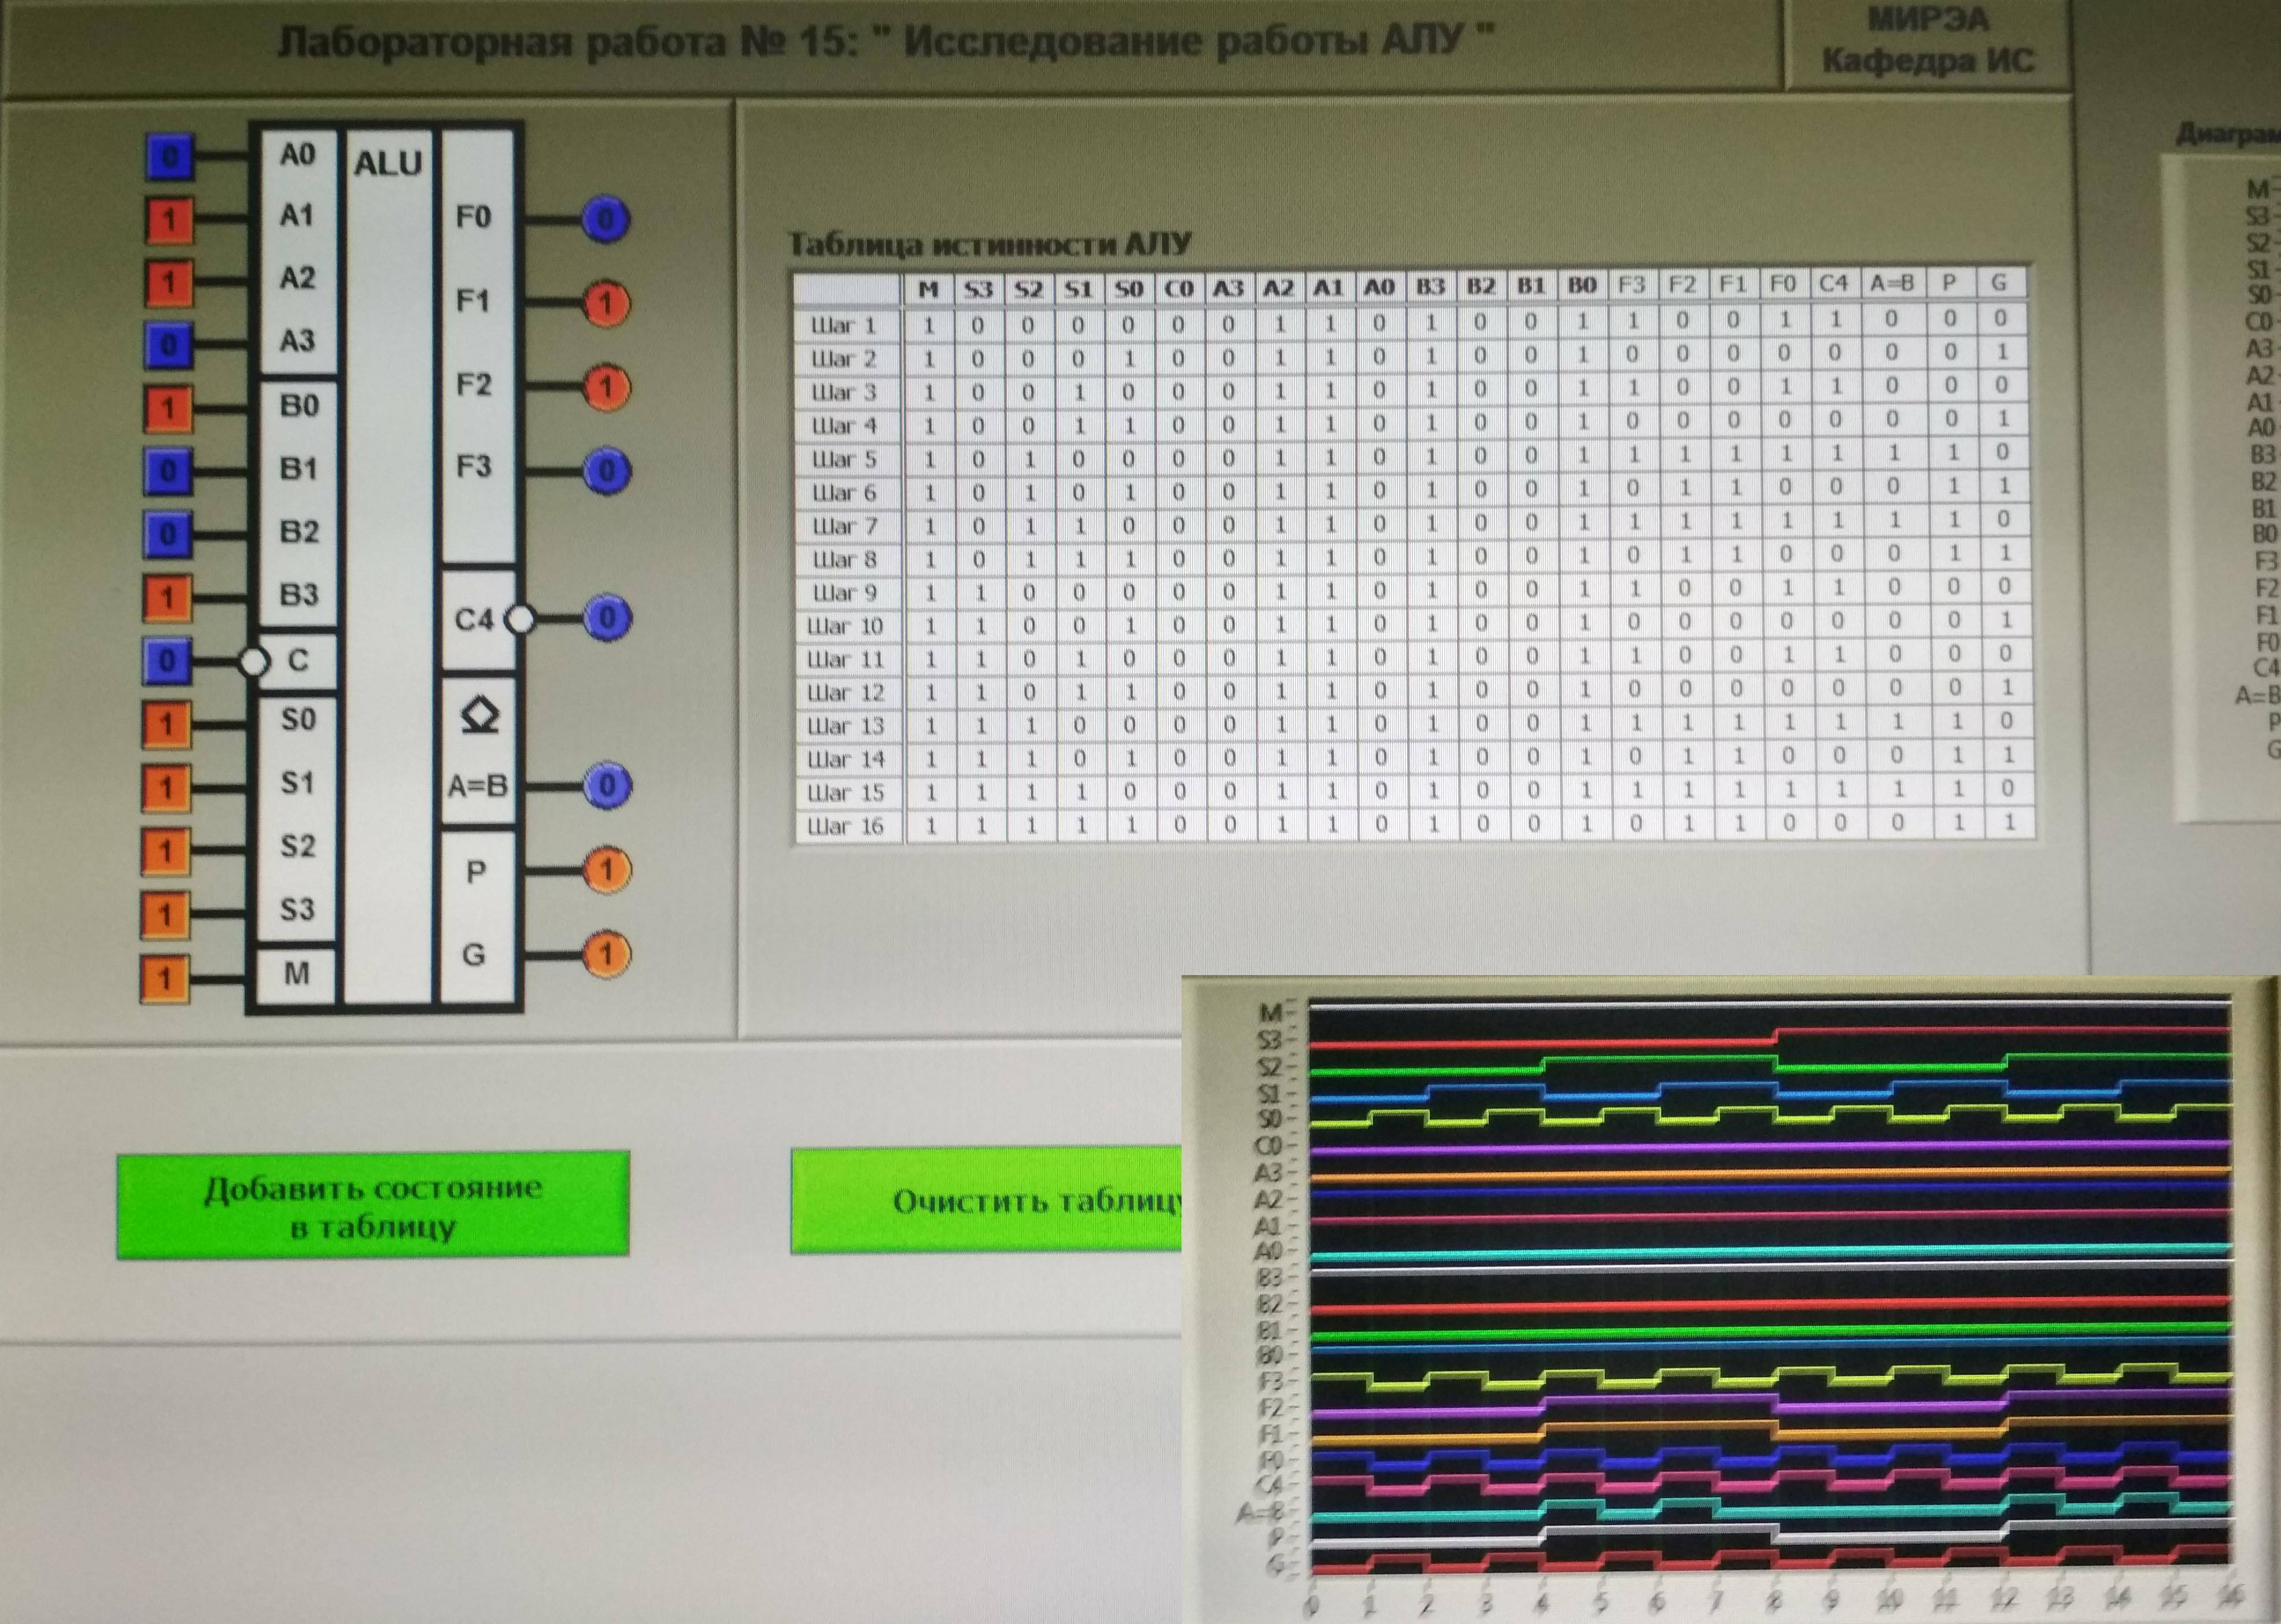
\includegraphics[width=0.95\linewidth]{imgs/15/1}
	\caption{Работа АЛУ в режиме выполнения логических операций}
	\label{fig:15_1}
\end{figure}

Работа АЛУ в режиме выполнения арифметических операций:

\begin{figure}[H]
	\centering
	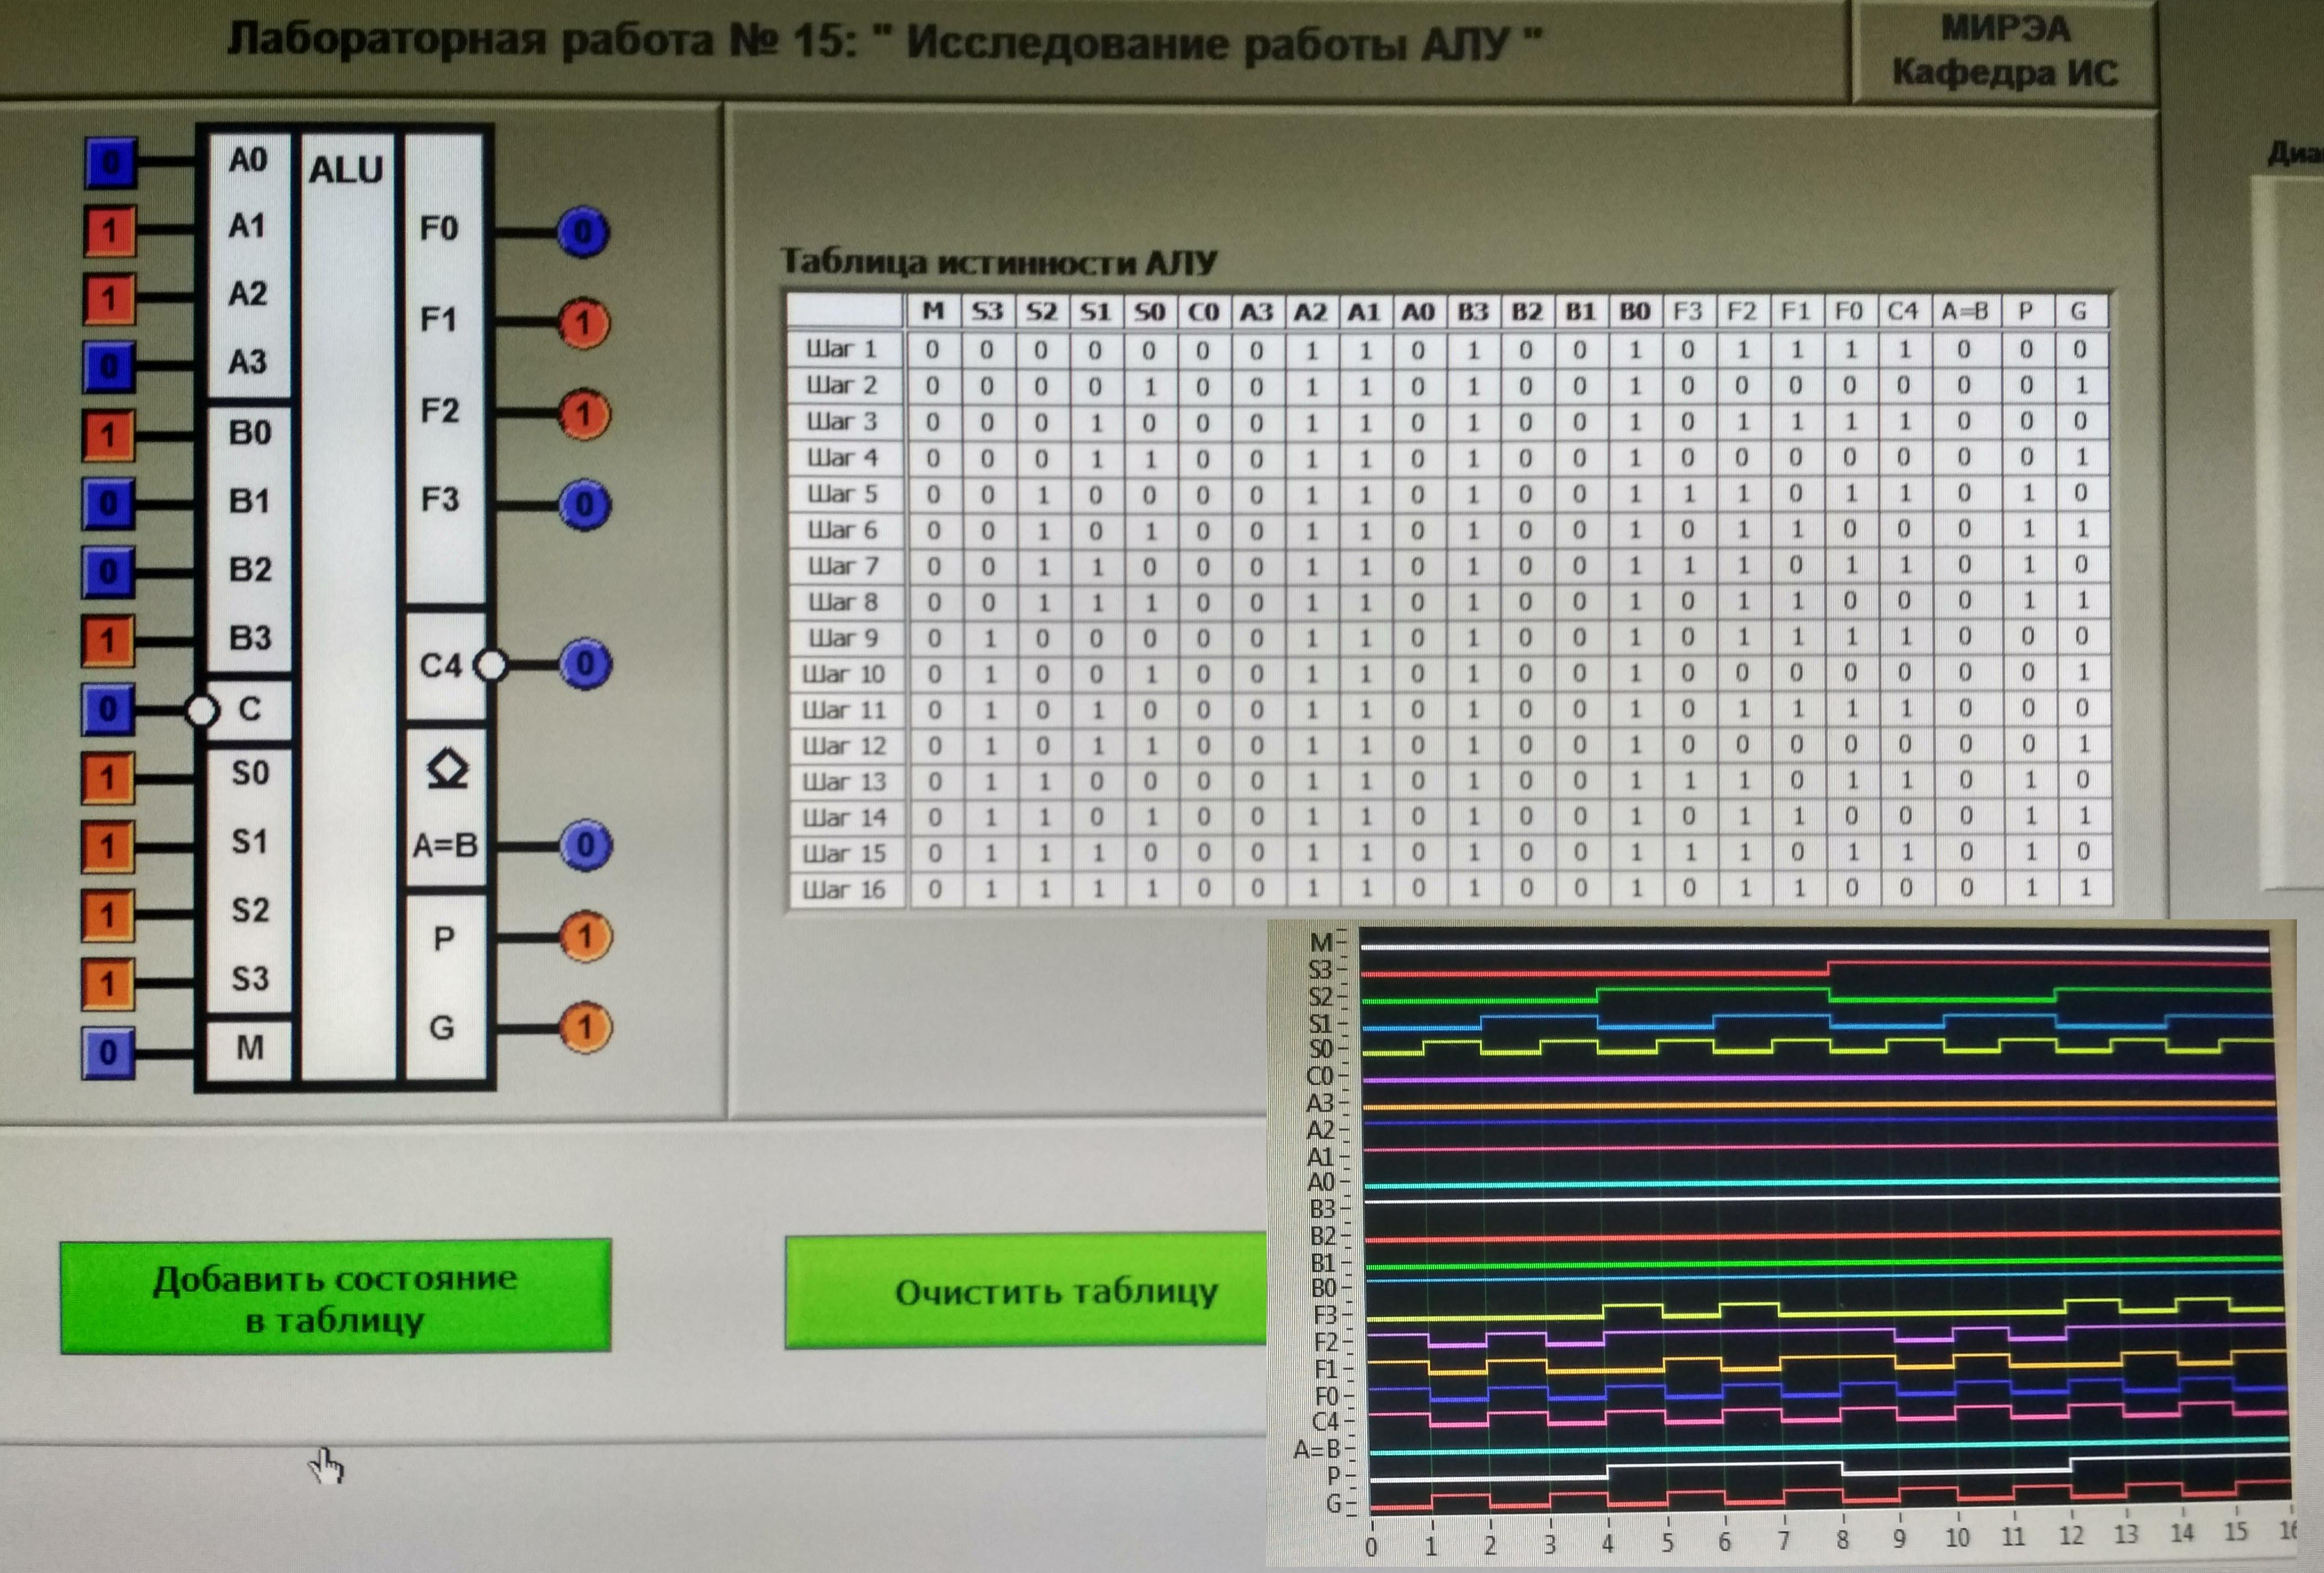
\includegraphics[width=0.95\linewidth]{imgs/15/2}
	\caption{ВЫПОЛНЕНИЕ АРИФМЕТИЧЕСКИХ ОПЕРАЦИЙ}
	\label{fig:15_2}
\end{figure}

\begin{figure}[H]
	\centering
	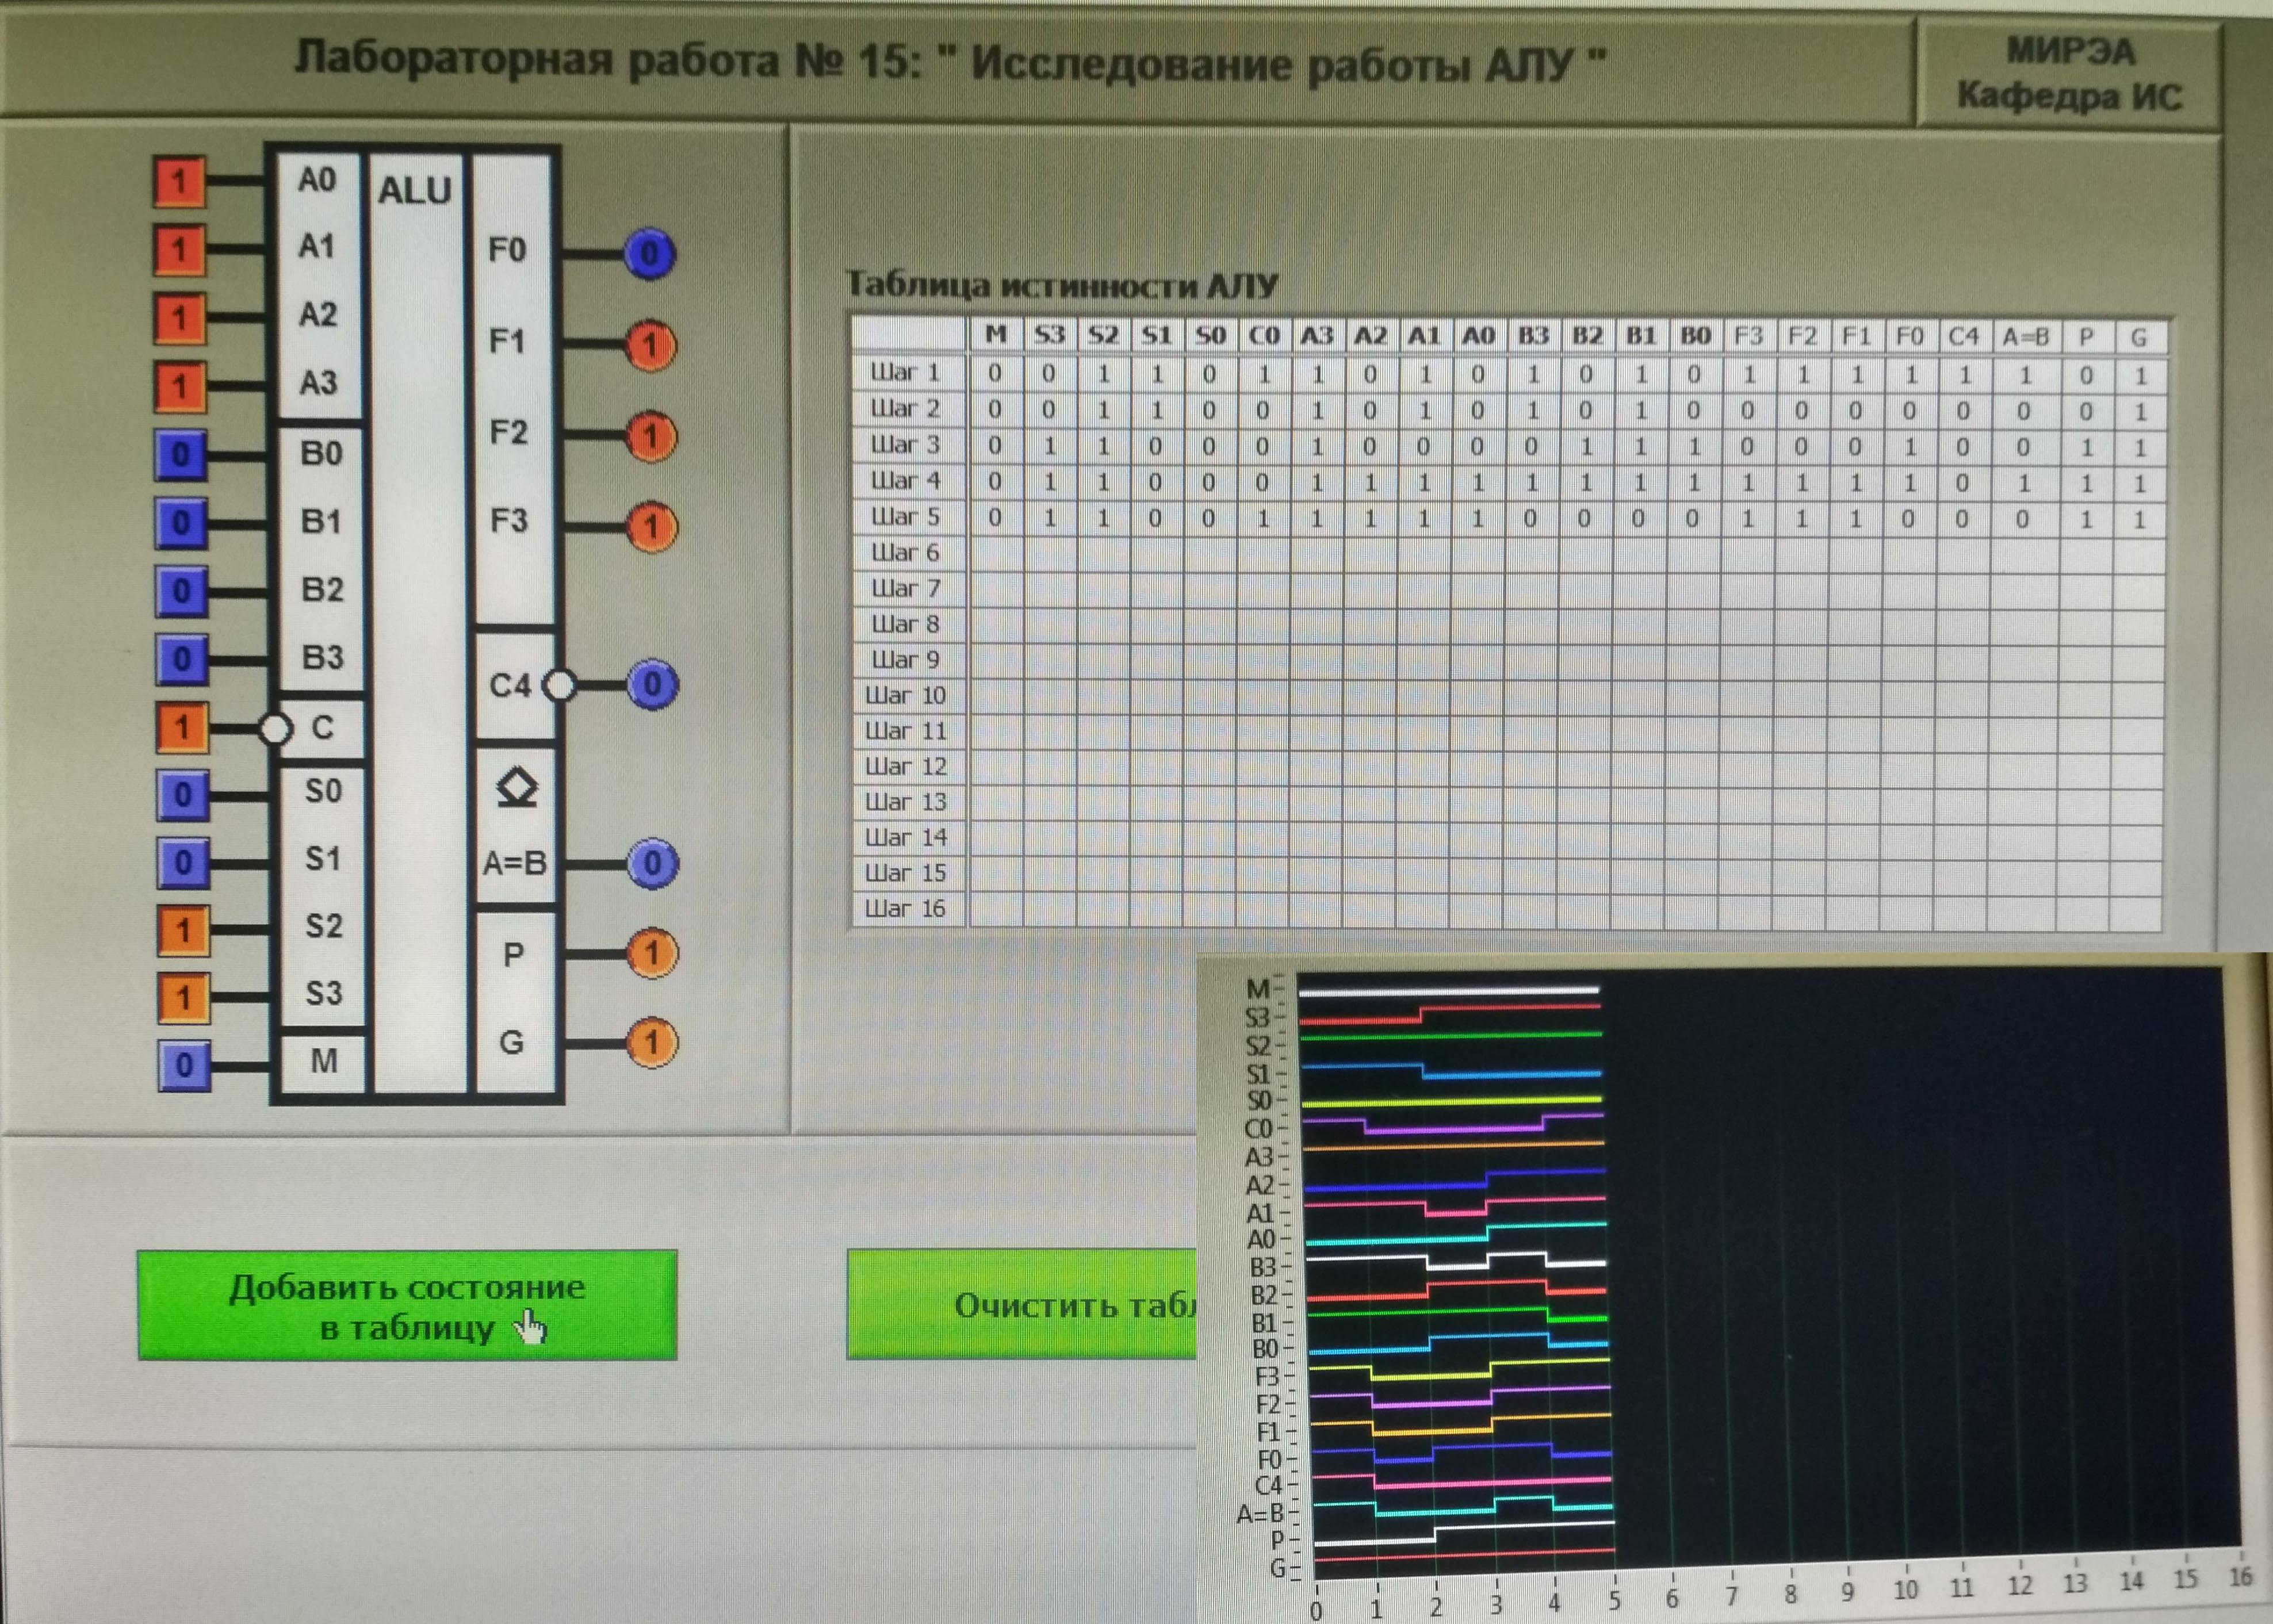
\includegraphics[width=0.95\linewidth]{imgs/15/3}
	\caption{РАБОТА СХЕМЫ СРАВНЕНИЯ И ПЕРЕНОСА}
	\label{fig:15_3}
\end{figure}

\begin{figure}[H]
	\centering
	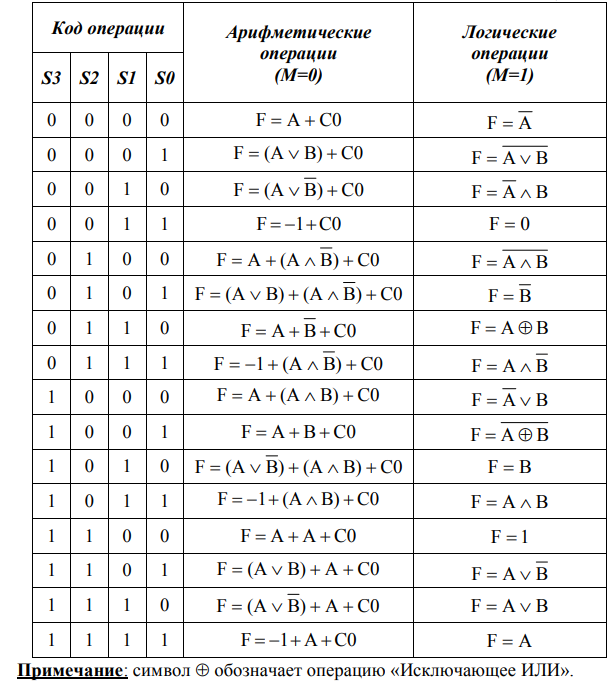
\includegraphics[width=0.85\linewidth]{imgs/15/15_tab}
	\caption{Режим работы АЛУ}
	\label{fig:15_tab}
\end{figure}

Элемент SN74LS181N - Schottky Logic

Характеристики:

\begin{figure}[H]
	\centering
	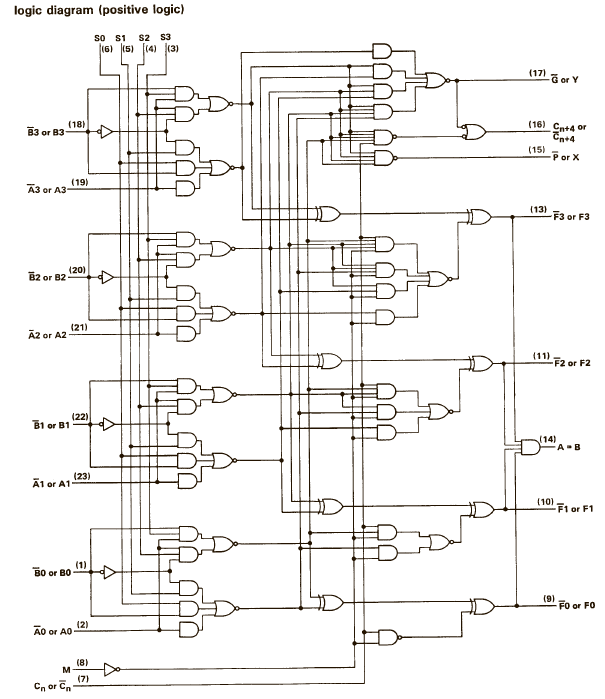
\includegraphics[width=0.95\linewidth]{imgs/15/15_sh}
	\caption{Схема}
	\label{fig:15_sh}
\end{figure}

\begin{figure}[H]
	\centering
	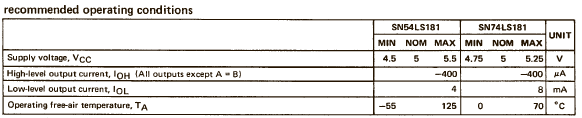
\includegraphics[width=0.95\linewidth]{imgs/15/15_rec}
	\caption{Рекомендуемые параметры}
	\label{fig:15_rec}
\end{figure}

\begin{figure}[H]
	\centering
	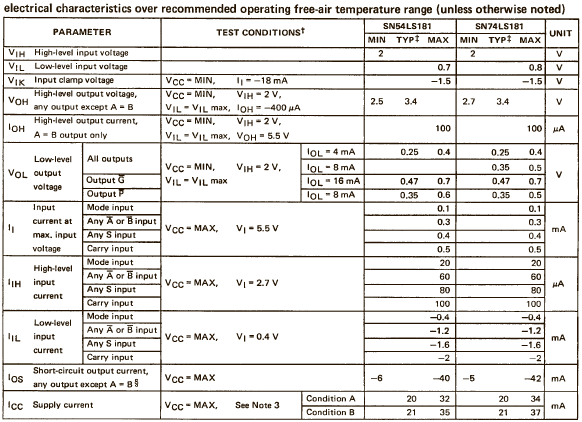
\includegraphics[width=0.95\linewidth]{imgs/15/15_el}
	\caption{Электрические характеристики}
	\label{fig:15_el}
\end{figure}

\begin{figure}[H]
	\centering
	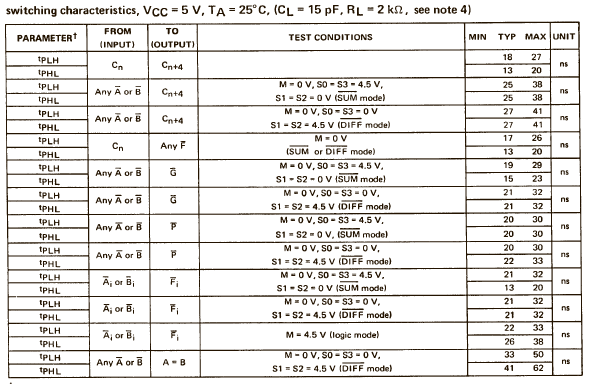
\includegraphics[width=0.95\linewidth]{imgs/15/15_switch}
	\caption{Коммутационные характеристики}
	\label{fig:15_switch}
\end{figure}
